%! suppress = UnresolvedReference


\chapter{相关技术介绍}\label{ch:tech}


\section{Flutter跨平台应用程序开发框架}\label{sec:flutter}

\subsection{使用跨平台应用程序开发框架的意义}\label{subsec:why-framework}

要开发一个\app ,首先要考虑的是该应用支持哪些移动平台。根据2023年3月的数据\cite{MobileOperatingSystem},在中国的移动平台操作系统占有率中,Android系统以76.15\%名列第一,iOS系统以23.28\%位居第二,这两个最主流的移动平台操作系统占据了绝大部分市场份额。因此,本应用开发的目标平台选定为Android和iOS。

Android和iOS开发的各种技术可以分为两大方向:原生应用程序开发和跨平台应用程序开发。构建传统的原生应用程序需要维护两个不同的代码库,分别为Android和iOS平台编写代码,通常意味着需要分别使用Kotlin/Java和Swift/Objective-C来编写两份高度相似的代码。而跨平台应用程序开发框架则可以通过一套代码库同时为Android和iOS平台构建应用程序,降低了开发人员的学习成本,缩减了开发时间,提高了开发效率。

\subsection{Flutter简介}\label{subsec:flutter}

Flutter是一个由Google开源的跨平台应用程序开发框架,仅通过一套代码库就能构建精美的、原生平台编译的跨平台应用\cite{FlutterBuildApps}。

Flutter对Android和iOS平台均有良好支持,此外还支持Windows、Linux、macOS、Web等平台\cite{SupportedDeploymentPlatforms}。基于Flutter框架进行开发不仅可以避免为Android和iOS平台分别编写大量相似的代码,还可以方便未来将部分不依赖于移动端特性的功能(比如历史心电展示等)的相关代码在其他平台(比如Web端)复用。

\subsection{Flutter与其他框架的对比}\label{subsec:flutter-compare}

Flutter并不是唯一一个支持Android和iOS平台的跨平台应用程序开发框架。在本项目的选型过程中也考虑了其他几个经常被与Flutter进行比较的同类框架,包括React Native\cite{ReactNativeLearn}、Xamarin\cite{XamarinOpensourceMobile}、Ionic Creator\cite{IonicFrameworkCrossPlatform}。

关于这几个框架,最先被对比的是其热度。以近一年的Google趋势作为标准,对比结果如图~\ref{fig:google-trends} 所示。

\begin{figure}[h]
    \centering
    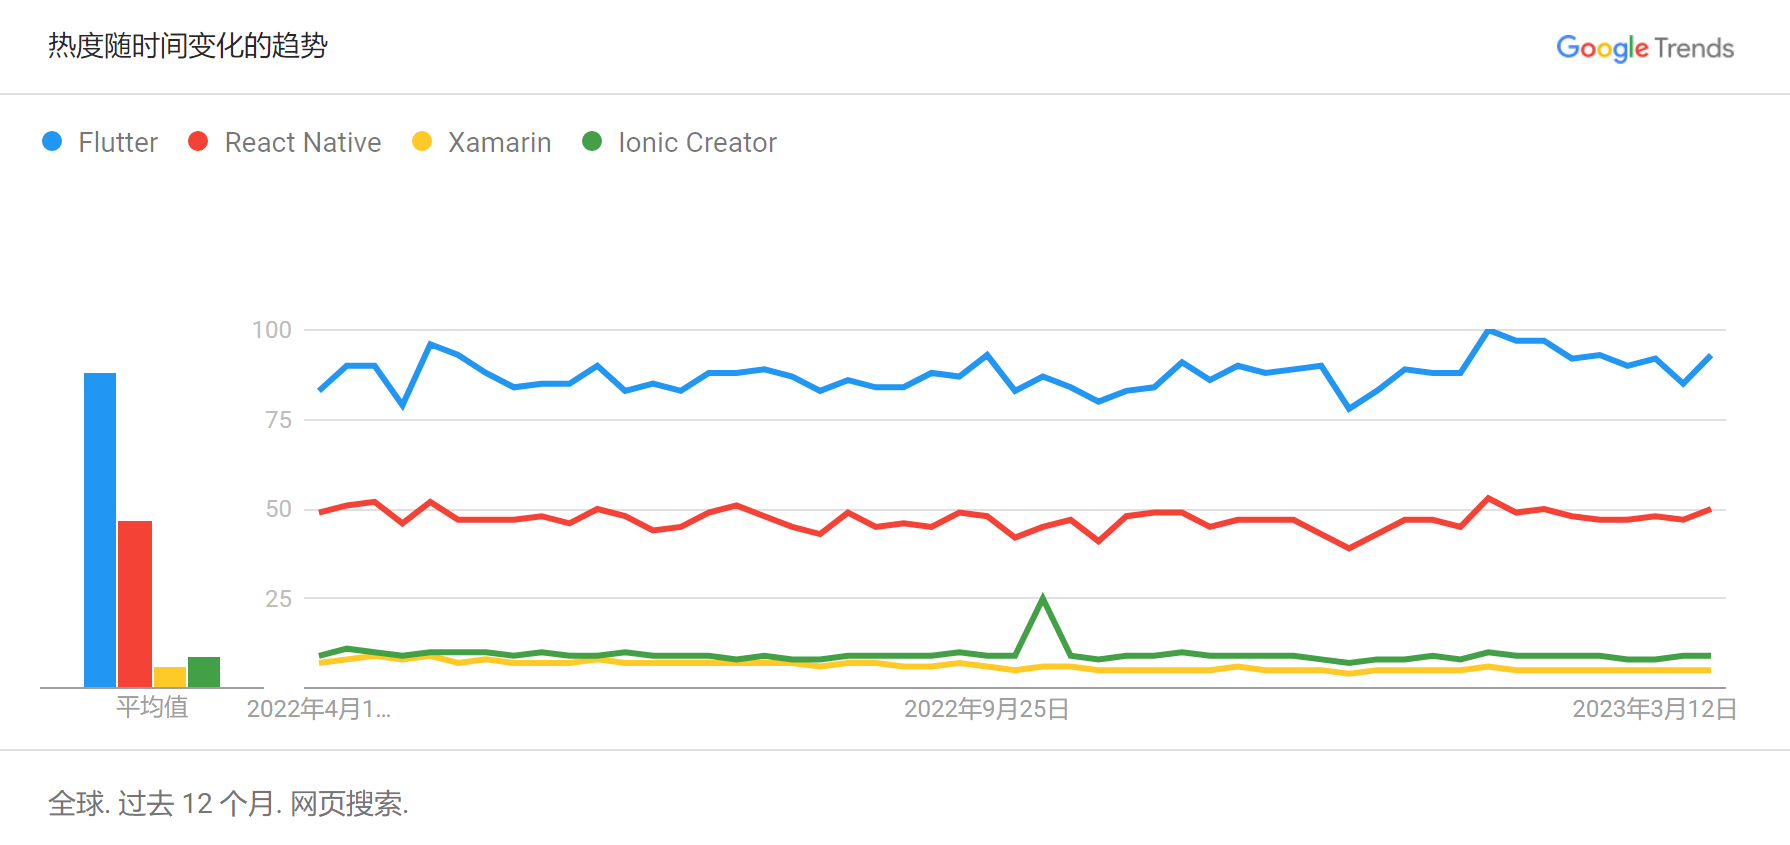
\includegraphics[width=\textwidth]{../assets/google-trends}
    \bicaption{Flutter与其他框架的Google趋势}{Google Trends for Flutter and other frameworks}
    \label{fig:google-trends}
\end{figure}

从图中可以看出,Flutter和React Native的热度远远高于Xamarin和Ionic Creator。热度高意味着其社区更加活跃,生态更为优秀,更容易找到相关的资料和技术支持,也更容易利用社区已经开发过的包,这些对于项目开发来说都是非常重要的。因此,Xamarin和Ionic Creator在本项目的选型过程中最先被排除。

之后需要对比的是Flutter和React Native。从热度上来看,两者的热度都比较平稳,Flutter长期保持在React Native的两倍左右,这意味着Flutter应当被优先考虑,但还不足以作为决定性理由。因此,需要进一步对比这两个框架的特性。

React Native是由Meta(前身为Facebook)于2015年开源的跨平台应用程序开发框架。正如其名称所暗示的,React Native和React(一个流行的Web框架)的关系十分密切,这既是优点也是缺点。从优点的方面来说,React Native非常适合已有React开发经验但没有移动平台开发经验的开发者快速上手,也适合将已有的基于React的Web项目迁移至移动端,但这两点对于本项目来说都没有明显意义。另一方面,由于和React的紧密联系,基于React Native的应用需要使用JavaScript和CSS编写,代码会在JavaScript引擎下解释执行,并通过序列化消息与本机代码桥接通信以渲染原生组件。JavaScript本来就不是一个以性能见长的语言,额外的桥接翻译层更使得其性能较之原生应用程序相去甚远。

作为对比,Flutter是Google于两年后(2017年)开源的,其设计上明显借鉴了React Native,与其一样使用响应式风格的界面编写方式。主要差别在于Flutter是编译成原生代码运行,直接接管并控制屏幕上的每一个像素,由此可以避免使用JavaScript桥接导致的性能问题。

除了上述的性能优势之外,Flutter还在热重载、IDE集成、内置调试工具等方面相较其他框架更为优秀。最终,基于以上所有考虑,本项目选择了Flutter作为开发框架。

\subsection{Dart语言}\label{subsec:dart}

Dart是由Google开源的编程语言,专门针对用户界面(User interface,缩写为UI)的创造进行优化,可编译为移动端、桌面端的二进制文件和Web平台的Javascript代码\cite{DartProgrammingLanguage}。Dart最初于2011年发布,原本是打算捆绑于Chrome浏览器来替代JavaScript,但后来由于各种因素而未能成功。在Flutter开发团队选择了Dart作为开发语言之后,两者的关系便愈加紧密,Dart也因此得到了更多的关注,并顺应Flutter框架的需求进行了许多更新迭代。时至今日,Dart与Flutter可以说是处于完全捆绑的状态,使用Flutter框架进行开发几乎是学习并使用Dart语言的唯一目的,使用Dart语言也是基于Flutter框架进行开发的必要条件。

Dart是一种多范式的语言,支持函数式、命令式、面向对象、反射式的写法,语法风格近似于C++与Java的混合,支持抽象类、泛型、类型推断、自动内存管理、空安全等其他语言中较为常见的特性,也有Mixin、Extension方法等其他语言中不太常见的特性。因篇幅限制,本文不便对Dart的诸多特性进行完整介绍,这里仅对后文必须涉及,且与其他语言有明显差异的部分特性进行简单说明。

\subsubsection{外部函数接口}\label{subsubsec:ffi}

外部函数接口(Foreign function interface,缩写为FFI)是一种机制,指用一种编程语言编写的程序可以调用另一种编程语言编写的功能。比如在C++中可以使用 \lstinline[language=C]{extern "C"} 来实现与C语言之间的双向FFI。

Dart作为一种专精于UI开发的语言,在其他方面的生态较为薄弱。作为一种弥补方式,Dart实现了与许多其他语言之间的FFI,比如在Web上可以与JavaScript互相调用,在macOS和iOS上可以与Swift和Objective-C互相调用,在Android、Windows、macOS、Linux上可以与Java和Kotlin互相调用,以及对本项目来说最重要的——在除Web以外的所有平台可以与C语言直接进行交互,而无须像React Native等框架那样通过Java等中间层进行间接调用,这使得Dart与C语言之间的FFI十分高效。由于C++代码也可以编译为C语言风格的接口,这意味着本应用的部分功能可以直接使用C++编写,从而充分利用C++的性能、生态、跨平台性等优势。

在项目的开发过程中,使用C++编写了两部分代码供Dart FFI调用,分别是Pan-Tompkins算法和基于LibTorch的人工智能算法,在后文会详细介绍。

\subsubsection{Isolate}\label{subsubsec:isolate}

Isolate是Dart中的一种介于线程与进程之间的概念。在Dart程序中,所有的代码都在Isolate中运行。每一个Isolate都有独立的运行线程和独立的堆内存,从而确保Isolate之间互相隔离,无法互相访问状态。相比于常规的线程,这样的实现并不会共享内存,所以也不需要担心互斥锁和其他锁等问题。相对地,由于无法与其他Isolate共享可变对象,Isolate之间的通信必须使用消息机制。

Dart程序有一个默认的主Isolate,在Flutter应用中也称为UI Isolate,因为UI的更新都是在主Isolate中进行的。在本应用中,数据库查询等可能较为耗时的操作都是放在其他Isolate中异步执行的,以避免阻塞UI Isolate导致UI卡顿。

\subsection{应用依赖的部分Flutter包}\label{subsec:flutter-packages}

\todo{依赖里有上百个包,介绍哪些?}


\section{项目使用的Python包与C++中的对应替代}\label{sec:python-cpp-packages}

\todo{为什么需要C++中的对应替代?(需要将Python算法迁移至C++,部分关键依赖无法消除。)}

\subsection{PyTorch与LibTorch}\label{subsec:pytorch-libtorch}

\todo{什么是PyTorch?}

\todo{什么是LibTorch?}

\todo{为什么选择LibTorch而不是MNN、NCNN等?(PyTorch官方支持,接口设计高度相似,引用官方文档中相关说明。)}

\subsection{NumPy与NumCpp}\label{subsec:numpy-numcpp}

\todo{什么是NumPy?}

\todo{什么是NumCpp?}

\todo{为什么选择NumCpp而不是Eigen等?(接口与NumPy更相似。)}

\subsection{pytest与Catch2}\label{subsec:pytest-catch2}

\todo{什么是pytest?(关于名字:pytest的官方名称即为全小写形式,即使在位于句首的情况下也是如此。)}

\todo{什么是Catch2?}

\todo{为什么选择Catch2而不是Google Test、Boost Test等?(更简单,本项目的C++部分没有编写复杂的测试用例的需求。)}

\subsection{nlohmann::json}\label{subsec:nlohmann-json}

\todo{为什么需要nlohmann::json?(Python标准库有JSON支持,C++没有,需要第三方库。)}

\todo{什么是nlohmann::json,不是其他JSON库?(接口简单。虽然性能有劣势,但只是用于读取少量测试数据,速度不重要。)}
